\chapter{जंतु कैसे जनन करते हैं}\label{ch:g4:animal-reproduction}

मई में तालाब मेंढकों के गान से गूँजता है; जून तक वह \omterm{ex:g2:animals-grow-up:frog}{टैडपोलों} से काला
पड़ जाता है। पता चलता है कि वह गान इसी कहानी की शुरुआत थी: जनन ---
यानी \omterm{def:g1:animals-around-us:animal}{जंतु} अगली पीढ़ी कैसे बनाते हैं --- ऐसे नियमों पर चलता है जो मेंढक
से लेकर हाथी तक टिके रहते हैं, और ब्यौरों में अद्भुत विविधता लिए रहते
हैं।

\section{इसमें दो लगते हैं}

\begin{definition}[लैंगिक जनन]\label{def:g4:animal-reproduction:sexual}
\omterm{def:g1:animals-around-us:animal}{जंतुओं} में बच्चे बनाने के लिए आम तौर पर दो जनक लगते हैं: एक
\emph{मादा}\index{मादा} और एक \emph{नर}\index{नर}। मादा
\emph{अंडाणु}\index{अंडाणु} बनाती है; नर
\emph{शुक्राणु}\index{शुक्राणु} बनाता है। नया \omterm{def:g1:animals-around-us:animal}{जंतु} तब शुरू होता है जब
एक शुक्राणु एक अंडाणु से जुड़ता है --- इसी जुड़ने को
\emph{निषेचन}\index{निषेचन} कहते हैं। दो जनकों वाले जनन को
\emph{लैंगिक जनन}\index{लैंगिक जनन} कहते हैं।
\end{definition}

\begin{example}[मेंढक क्यों गाते हैं]\label{ex:g4:animal-reproduction:song}
मई का समवेत गान नरों का \omterm{def:g4:animal-reproduction:sexual}{मादाओं} को तालाब बुलाना है। फिर हर जोड़ी अपनी
कोशिकाएँ पानी में छोड़ती है --- \omterm{def:g4:animal-reproduction:sexual}{मादा} के \omterm{def:g2:animals-grow-up:born}{अंडे}, \omterm{def:g4:animal-reproduction:sexual}{नर} के \omterm{def:g4:animal-reproduction:sexual}{शुक्राणु} --- और
वहीं \omterm{def:g4:animal-reproduction:sexual}{निषेचन} होता है। कुछ दिन बाद लुआब में दिखते काले बिंदु पहले से बढ़
रहे बच्चे हैं: वह गान \cref{ch:g2:animals-grow-up} वाले मेंढक-चक्र का
पहला क़दम था।
\end{example}

\begin{omfigure}
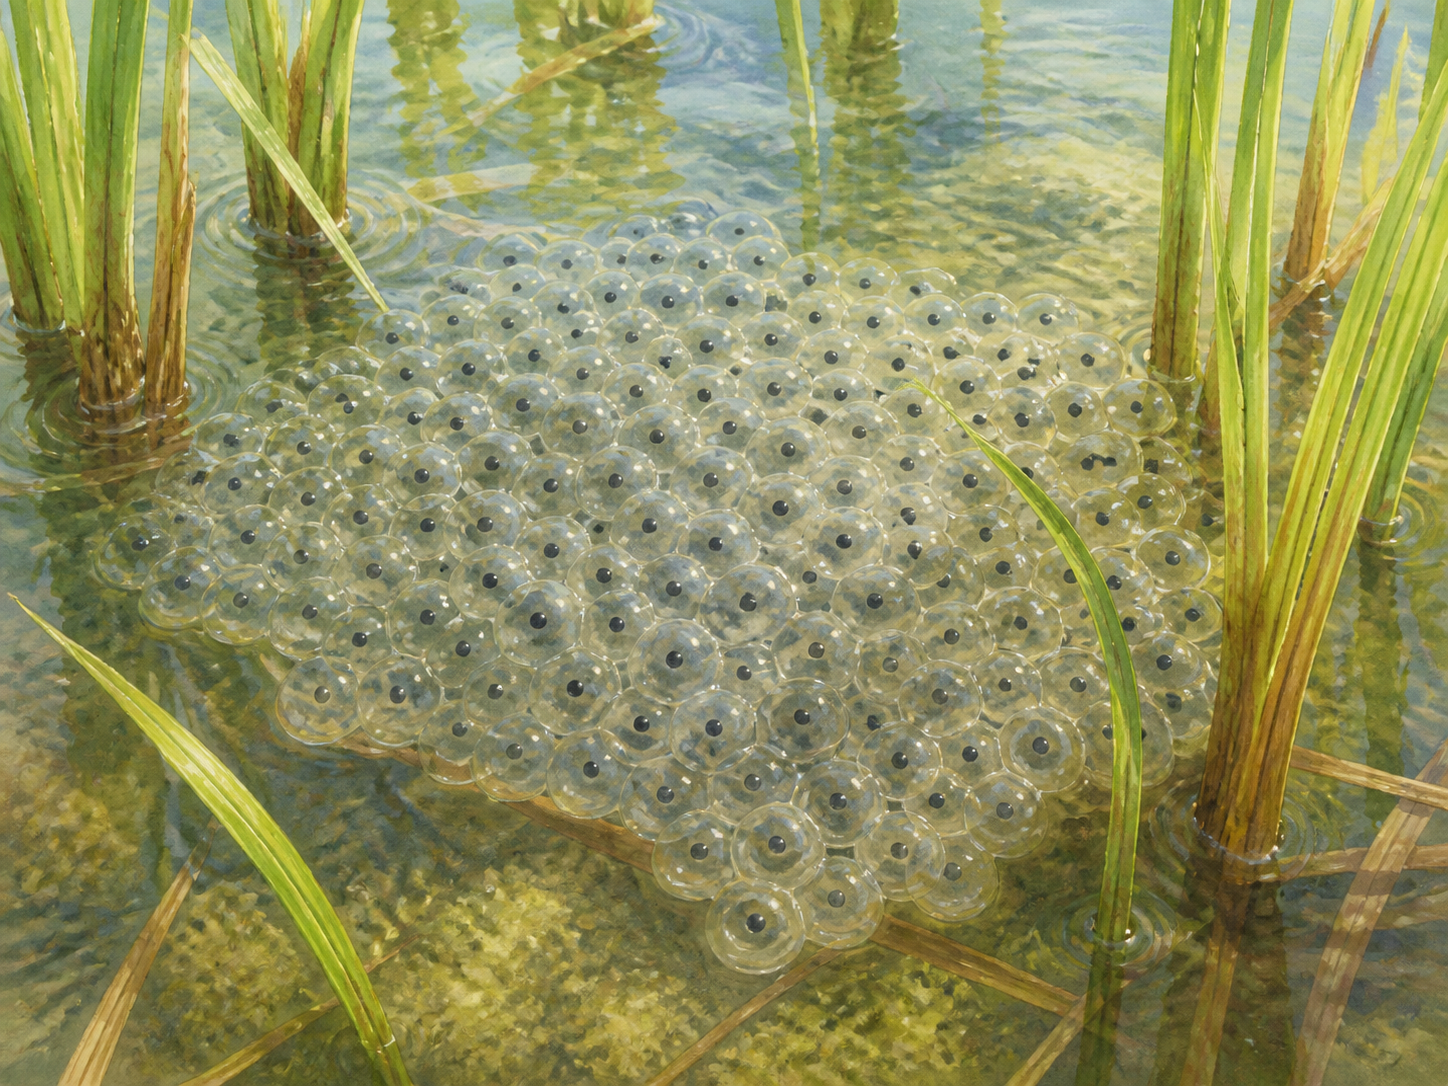
\includegraphics[width=0.56\linewidth]{images/book1/ai/g4-repro-frogspawn.png}

{\small गान के कुछ दिन बाद: सरकंडों के बीच मेंढक के \omterm{def:g2:animals-grow-up:born}{अंडे}, और लुआब का
हर गोला एक निषेचित \omterm{def:g2:animals-grow-up:born}{अंडा}, जिसके भीतर एक नन्हा मेंढक शुरू हो चुका है।}
\end{omfigure}

\begin{remark}[दो जनक, मिली-जुली क़िस्मत]\label{rem:g4:animal-reproduction:mix}
नया \omterm{def:g1:animals-around-us:animal}{जंतु} हर जनक से कुछ न कुछ पाता है --- इसीलिए किसी बछेड़े का रंग अपनी
माँ जैसा और माथे की सफ़ेद धारी अपने पिता जैसी हो सकती है। हर जनक
ठीक-ठीक क्या सौंपता है, और कैसे, यह इस पुस्तक के आगे के बड़े सवालों
में से एक है; फ़िलहाल बस इतना ध्यान रखो कि \omterm{def:g4:animal-reproduction:sexual}{लैंगिक जनन} से बने हर \omterm{def:g1:animals-around-us:animal}{जंतु}
के दो जनक होते हैं और वह दोनों जैसा दिखता है।
\end{remark}

\section{अंडे दिए गए, या बच्चे जीवित जन्मे}

\begin{definition}[अंडज और जरायुज]\label{def:g4:animal-reproduction:ovivivi}
\Cref{def:g2:animals-grow-up:born} के जन्म के दोनों ढंगों को अब उनके
वैज्ञानिक नाम मिलते हैं:
\begin{itemize}
  \item \omterm{def:g1:animals-around-us:animal}{जंतु} \emph{अंडज}\index{अंडज} है अगर \omterm{def:g4:animal-reproduction:sexual}{मादा} \emph{\omterm{def:g2:animals-grow-up:born}{अंडे}} देती है,
        और बच्चे \omterm{def:g2:animals-grow-up:born}{अंडे} के भीतर, उसके शरीर के बाहर बढ़कर पूरे होते हैं:
        \omterm{prop:g3:sorting-living-things:groups}{पक्षी}, ज़्यादातर \omterm{prop:g3:sorting-living-things:groups}{मछलियाँ}, ज़्यादातर \omterm{prop:g4:classifying-animals:classes}{सरीसृप}, \omterm{prop:g3:sorting-living-things:groups}{उभयचर}, \omterm{prop:g3:sorting-living-things:groups}{कीट},
        घोंघे;
  \item \omterm{def:g1:animals-around-us:animal}{जंतु} \emph{जरायुज}\index{जरायुज} है अगर बच्चा \emph{माँ के
        शरीर के भीतर} बढ़ता है, उसी से पोषण पाता है, और
        \emph{\omterm{def:g2:animals-grow-up:born}{जीवित जन्म}} लेता है: लगभग सारे \omterm{prop:g3:sorting-living-things:groups}{स्तनधारी}।
\end{itemize}
\end{definition}

\begin{example}[दो पालनाघर]\label{ex:g4:animal-reproduction:nurseries}
मुर्ग़ी का चूज़ा तीन गरम हफ़्ते खोलदार \omterm{def:g2:animals-grow-up:born}{अंडे} में बिताता है और ज़र्दी पर
जीता है (\cref{rem:g2:animals-grow-up:egg}); बछेड़ा ग्यारह महीने घोड़ी
के भीतर बिताता है, लगातार उसके शरीर से पोषण पाता है, और जन्म के घंटे
भर में खड़े होने लायक़ पैदा होता है। लक्ष्य वही, पालनाघर दो: एक में
\omterm{def:g1:animals-around-us:covering}{खोल} में बँधा भोजन, दूसरे में भीतर से लगातार सेवा।
\end{example}

\begin{proposition}[निषेचन कहाँ होता है]\label{prop:g4:animal-reproduction:where}
\omterm{prop:g3:sorting-living-things:groups}{मछलियों} और मेंढकों जैसे पानी में रहने वालों में \omterm{def:g4:animal-reproduction:sexual}{निषेचन} आम तौर पर
\emph{पानी में}, \omterm{def:g4:animal-reproduction:sexual}{मादा} के शरीर के बाहर होता है --- \omterm{def:g2:animals-grow-up:born}{अंडे} और \omterm{def:g4:animal-reproduction:sexual}{शुक्राणु}
साथ-साथ छोड़े जाते हैं और हज़ारों की तादाद में मिलते हैं। ज़मीन के
\omterm{def:g1:animals-around-us:animal}{जंतुओं} में --- \omterm{prop:g3:sorting-living-things:groups}{पक्षी}, \omterm{prop:g4:classifying-animals:classes}{सरीसृप}, \omterm{prop:g3:sorting-living-things:groups}{स्तनधारी}, \omterm{prop:g3:sorting-living-things:groups}{कीट} --- ये कोशिकाएँ खुले में
सूख जातीं, इसलिए \omterm{def:g4:animal-reproduction:sexual}{नर} अपने \omterm{def:g4:animal-reproduction:sexual}{शुक्राणु} \emph{\omterm{def:g4:animal-reproduction:sexual}{मादा} के शरीर के भीतर}
\emph{समागम}\index{समागम} के दौरान पहुँचाता है, और \omterm{def:g4:animal-reproduction:sexual}{निषेचन} वहीं होता
है।
\end{proposition}
\admitted

\section{कम बच्चे और ख़ूब देखभाल, या बहुत बच्चे और कोई नहीं}

\begin{proposition}[अगली पीढ़ी के लिए दो रणनीतियाँ]\label{prop:g4:animal-reproduction:strategies}
गिनती की तुलना करो: कॉड मछली साल में \emph{लाखों} \omterm{def:g2:animals-grow-up:born}{अंडे} छोड़ती है और
किसी की देखभाल नहीं करती; हथिनी हर कुछ सालों में \emph{एक} बच्चा जनती
है और एक दशक तक उसकी रखवाली करती है। इन दोनों सिरों के बीच जंतु-जगत भर
में एक नियम टिकता है: प्रजाति जितने ज़्यादा बच्चे पैदा करती है, हर एक
को उतनी ही कम देखभाल मिलती है --- और जितने कम पैदा करती है, हर एक की
उतनी ही ज़्यादा रक्षा और पोषण होता है। दोनों रणनीतियाँ सफल हैं: औसतन
इतने बच्चे बच जाते हैं कि जनकों की जगह ले सकें।
\end{proposition}
\admitted

\begin{example}[तालाब की गिनती]\label{ex:g4:animal-reproduction:pondcount}
मेंढक की एक जोड़ी के गुच्छे में हज़ारों \omterm{def:g2:animals-grow-up:born}{अंडे} होते हैं। बगुले,
काँटा-मछलियाँ और व्याध-पतंगों के डिंभ (देखो
\cref{ex:g3:food-chains:three}) पूरे वसंत \omterm{ex:g2:animals-grow-up:frog}{टैडपोल} खाते रहते हैं ---
और हज़ारों में से गिनती के कुछ नन्हे मेंढक जुलाई में किनारे चढ़ते हैं।
वह विशाल गुच्छा बरबादी नहीं है: बिना किसी जनक-पहरे के, तालाब के ख़तरों
का मेंढक का यही उत्तर है।
\end{example}

\begin{example}[दूसरा सिरा]\label{ex:g4:animal-reproduction:whalecalf}
ह्वेल का बच्चा अकेला जन्म लेता है, तुरंत अपनी माँ के साथ तैरने लगता
है, कई महीने उसका गाढ़ा \omterm{def:g2:animals-grow-up:born}{दूध} पीता है और हर ख़तरे से उसकी रक्षा की जाती
है। एक बार में एक ही बच्चा --- पर उस एक को सब कुछ मिलता है। अपने \omterm{def:g2:animals-grow-up:born}{दूध}
के साथ (\cref{def:g2:animals-grow-up:born}) \omterm{prop:g3:sorting-living-things:groups}{स्तनधारी}
कम-और-देखभाल-वाली रणनीति के सबसे बड़े विशेषज्ञ हैं।
\end{example}

\begin{method}[किसी प्रजाति की रणनीति पढ़ना]\label{met:g4:animal-reproduction:read}
कोई प्रजाति सामने हो, तो पूछो:
\begin{enumerate}
  \item एक बार में कितने बच्चे --- एक, दर्जन भर, हज़ारों?
  \item उनकी रखवाली और पोषण कौन करता है --- दोनों जनक, माँ, या कोई
        नहीं?
  \item वे शुरू कहाँ होते हैं --- बाहर \omterm{def:g2:animals-grow-up:born}{अंडे} में, या भीतर बढ़ते हुए?
  \item \cref{prop:g4:animal-reproduction:strategies} का संतुलन
        जाँचो: बहुत बच्चे और थोड़ी देखभाल, या कम बच्चे और ख़ूब
        देखभाल।
\end{enumerate}
\end{method}

\section{अभ्यास}

\begin{exercise}[$\star$]\label{exo:g4:animal-reproduction:1}
\omterm{def:g4:animal-reproduction:sexual}{निषेचन} क्या है? हर जनक से कौन-सी कोशिका आती है?
\end{exercise}

\begin{exercise}[$\star$]\label{exo:g4:animal-reproduction:2}
\omterm{def:g4:animal-reproduction:ovivivi}{अंडज} और \omterm{def:g4:animal-reproduction:ovivivi}{जरायुज} की परिभाषा दो, और हर तरह के दो-दो \omterm{def:g1:animals-around-us:animal}{जंतु} भी बताओ।
\end{exercise}

\begin{exercise}[$\star$]\label{exo:g4:animal-reproduction:3}
मई में मेंढक क्यों गा रहे थे? तालाब की कहानी तीन क़दमों में दोहराओ।
\end{exercise}

\begin{exercise}[$\star$]\label{exo:g4:animal-reproduction:4}
ट्राउट का \omterm{def:g4:animal-reproduction:sexual}{निषेचन} कहाँ होता है, और मुर्ग़ी का कहाँ?
\cref{prop:g4:animal-reproduction:where} के अनुसार यह फ़र्क़ क्यों है?
\end{exercise}

\begin{exercise}[$\star$]\label{exo:g4:animal-reproduction:5}
चूज़े और बछेड़े के पालनाघरों की तुलना करो: हर एक कहाँ बढ़ता है, और उसे
क्या खिलाता है?
\end{exercise}

\begin{exercise}[$\star$]\label{exo:g4:animal-reproduction:6}
बच्चों की संख्या और उन्हें मिलने वाली देखभाल को जोड़ने वाला नियम बताओ।
अध्याय के दोनों सिरों के उदाहरण दो।
\end{exercise}

\begin{exercise}[$\star$]\label{exo:g4:animal-reproduction:7}
कॉड मछली के लाखों \omterm{def:g2:animals-grow-up:born}{अंडों} में से ज़्यादातर कभी वयस्क कॉड नहीं बनते। फिर
भी यह रणनीति सफल क्यों है?
\end{exercise}

\begin{exercise}[$\star$]\label{exo:g4:animal-reproduction:8}
बिल्ली पर \cref{met:g4:animal-reproduction:read} चलाओ: आम तौर पर लगभग
पाँच बच्चे, माँ हफ़्तों तक \omterm{def:g2:animals-grow-up:born}{दूध} पिलाती और रखवाली करती है, और वे उसी के
भीतर बढ़े थे। वह रणनीति के किस पक्ष के ज़्यादा पास है?
\end{exercise}

\begin{exercise}[$\star\star$]\label{exo:g4:animal-reproduction:9}
बछेड़ा अकसर अपने दोनों जनकों जैसा एक साथ दिखता है।
\cref{rem:g4:animal-reproduction:mix} के अनुसार इससे पता चलता है कि
बच्चे को क्या मिलता है?
\end{exercise}

\begin{exercise}[$\star\star$]\label{exo:g4:animal-reproduction:10}
काँटा-मछली का \omterm{def:g4:animal-reproduction:sexual}{नर} घोंसला बनाता है, \omterm{def:g2:animals-grow-up:born}{अंडों} पर पानी हिलाता है और घुसपैठियों
को भगाता है --- मछली के लिए दुर्लभ समर्पण।
\cref{prop:g4:animal-reproduction:strategies} से तुम कॉड मछली के
लाखों के मुक़ाबले उसके गुच्छे के आकार के बारे में क्या भविष्यवाणी
करोगे?
\end{exercise}

\begin{exercise}[$\star\star\star$]\label{exo:g4:animal-reproduction:11}
समुद्री कछुए अपने \omterm{def:g2:animals-grow-up:born}{अंडे} गरम रेत में गाड़ने के लिए किनारे पर रेंगकर आते
हैं, और फिर समुद्र लौट जाते हैं। \omterm{def:g4:animal-reproduction:ovivivi}{अंडज} या \omterm{def:g4:animal-reproduction:ovivivi}{जरायुज}? देखभाल होती है या
नहीं? और यह \omterm{prop:g4:classifying-animals:classes}{सरीसृप}, जो जीवन भर तैरता है, फिर भी \emph{ज़मीन} पर ही
\omterm{def:g2:animals-grow-up:born}{अंडे} क्यों देता है? (\cref{prop:g4:classifying-animals:classes} की
\omterm{prop:g4:classifying-animals:classes}{सरीसृप} ख़ासियतें काम में लो।)
\end{exercise}
